\documentclass{article}
% ready for submission
\usepackage[preprint]{neurips_2023}
\usepackage{biblatex} %Imports biblatex package
\addbibresource{sample.bib} %Import the bibliography file
\usepackage{graphicx}

% to compile a preprint version, e.g., for submission to arXiv, add add the
% [preprint] option:
%\usepackage[preprint]{neurips_2023}


% to compile a camera-ready version, add the [final] option, e.g.:
%     \usepackage[final]{neurips_2023}


% to avoid loading the natbib package, add option nonatbib:
%    \usepackage[nonatbib]{neurips_2023}


\usepackage[utf8]{inputenc} % allow utf-8 input
\usepackage[T1]{fontenc}    % use 8-bit T1 fonts
\usepackage{hyperref}       % hyperlinks
\usepackage{url}            % simple URL typesetting
\usepackage{booktabs}       % professional-quality tables
\usepackage{amsfonts}       % blackboard math symbols
\usepackage{nicefrac}       % compact symbols for 1/2, etc.
\usepackage{microtype}      % microtypography
\usepackage{xcolor}         % colors


\title{Image Recovery From Underexposed Photographs Using Generative Models}

\author{
  Moises Lopez \\
  Department of Electrical & Computer Engineering \\
  University of Califonia San Diego \\
  % La Jolla, CA 92093 \\
  \texttt{mlopezme@ucsd.edu} \\
  % examples of more authors
  \And
  Sepehr Aiden Bostan \\
  Department of Electrical & Computer Engineering \\
  University of Califonia San Diego \\
  % La Jolla, CA 92093 \\
  \texttt{sbostanb@ucsd.edu} \\
  \And
  Yiteng Zhao \\
  Department of Electrical & Computer Engineering \\
  University of Califonia San Diego \\
  % La Jolla, CA 92093 \\
  \texttt{yiz097@ucsd.edu}
}


\begin{document}


\maketitle
\begin{abstract}
  Low light imagery has been a persistent challenge in fields like photography, computer vision, and feature detection. To address this problem, probabilistic methods and deep generative models such as GANs have emerged as promising solutions. In this paper, we present our approach to recovering underexposed images using GAN-based techniques, while also addressing the shortcomings of existing methods. Our proposed approach improves the quality of recovered images, making them more visually appealing and useful in various applications such as object detection in low light using cameras or simply photography in extremely dark conditions.
\end{abstract}



\section{Introduction}
\subsection{What research problem are we trying to solve?}
Social media and computer vision applications demand high-quality images, but current CMOS sensors used in cameras and smartphones struggle to perform well in challenging lighting conditions due to physical limitations. Low levels of photons captured by CMOS pixels result in dark, under-exposed images that are difficult for both computer analysis and human perception. Traditional physical methods such as enlarging pixels, aperture or increasing ISO can improve the Signal-to-Noise ratio, but at the cost of resolution, depth of field, or noise in the image. Therefore, our research aims to develop a better computational approach using a probabilistic neural network model to recover under-exposed images while maintaining their sharpness, color accuracy, and cleanliness.

\subsection{Why is this problem important?}
The potential of solving this problem can extend from mere convenience to saving lives. For example, in computer vision and autonomous vehicles, instead of using lidars in low light conditions we can simply use cameras for object detection and obstacle avoidance. Similarly, in search and rescue operations, a similar method can be used. In radiation imagery such as x-ray images used in the medical field, underexposed pixels can result in a loss of crucial details, potentially hiding a small tumor or other irregularities that would otherwise be detected by medical professionals. On the other hand, in photography, underexposed images can be recreated with higher brightness, which can merely be convenient for people.
\section{Related Works}

The literature has thoroughly examined the computational processing of low-light images. We will give a brief overview of the methods currently available.

\subsubsection{Convolutional Neural Networks} 
Researchers have explored the use of deep neural networks for extreme low-light imaging, but the approach has limitations and shortcomings. One issue is that the convolutional network\cite{LearningToSeeInTheDark} is individually tuned for each camera sensor, requiring cross-sensor generalization to be effective across different cameras. The hyper-parameters of the network, such as amplification factors, also need to be manually tuned, indicating the need for an auto ISO feature to improve efficiency. Additionally, the absence of HDR tone mapping and dynamic objects in the dataset limits the network's ability to enhance such images. Artifacts in the final image could also potentially be reduced. Finally, the long processing time of 0.38-0.66 seconds per image could be problematic for real-time applications. These limitations need to be addressed to improve the practicality and effectiveness of deep neural networks for image enhancement.

\subsubsection{Low-light image enhancement.}

There are different techniques for image enhancement, including histogram equalization and gamma correction. Histogram equalization involves balancing the histogram of the entire image, while gamma correction increases the brightness of dark regions and compresses bright pixels. More advanced techniques involve global analysis and processing, such as the inverse dark channel prior, wavelet transform \cite{AutomaticContrastEnhancement}, Retinex model\cite{retinex}, and illumination map estimation\cite{illumest}. However, these techniques typically assume that the images already have a good representation of the scene content.

However, we are focusing on extreme low-light imaging, which is characterized by high levels of noise and color distortion that exceed the capabilities of current enhancement pipelines.

\section{Methodology}
%\subsection{Proposed a solution for solving this problem}
We propose a generative network model that our generative network is designed to analyze and sample from the distribution of under-exposed images, and generate well-exposed images for comparing against the discriminate network using CNNs with ground truth as input. 
\section{Novelty and significance of our solution}
Our solution increases the quality and usability of underexposed images which are common in various applications. As mentioned before the potential of solving this problem can extend from mere convenience to saving lives.
\section{Tentative timeline}
\begin{figure}[h]
  \centering
  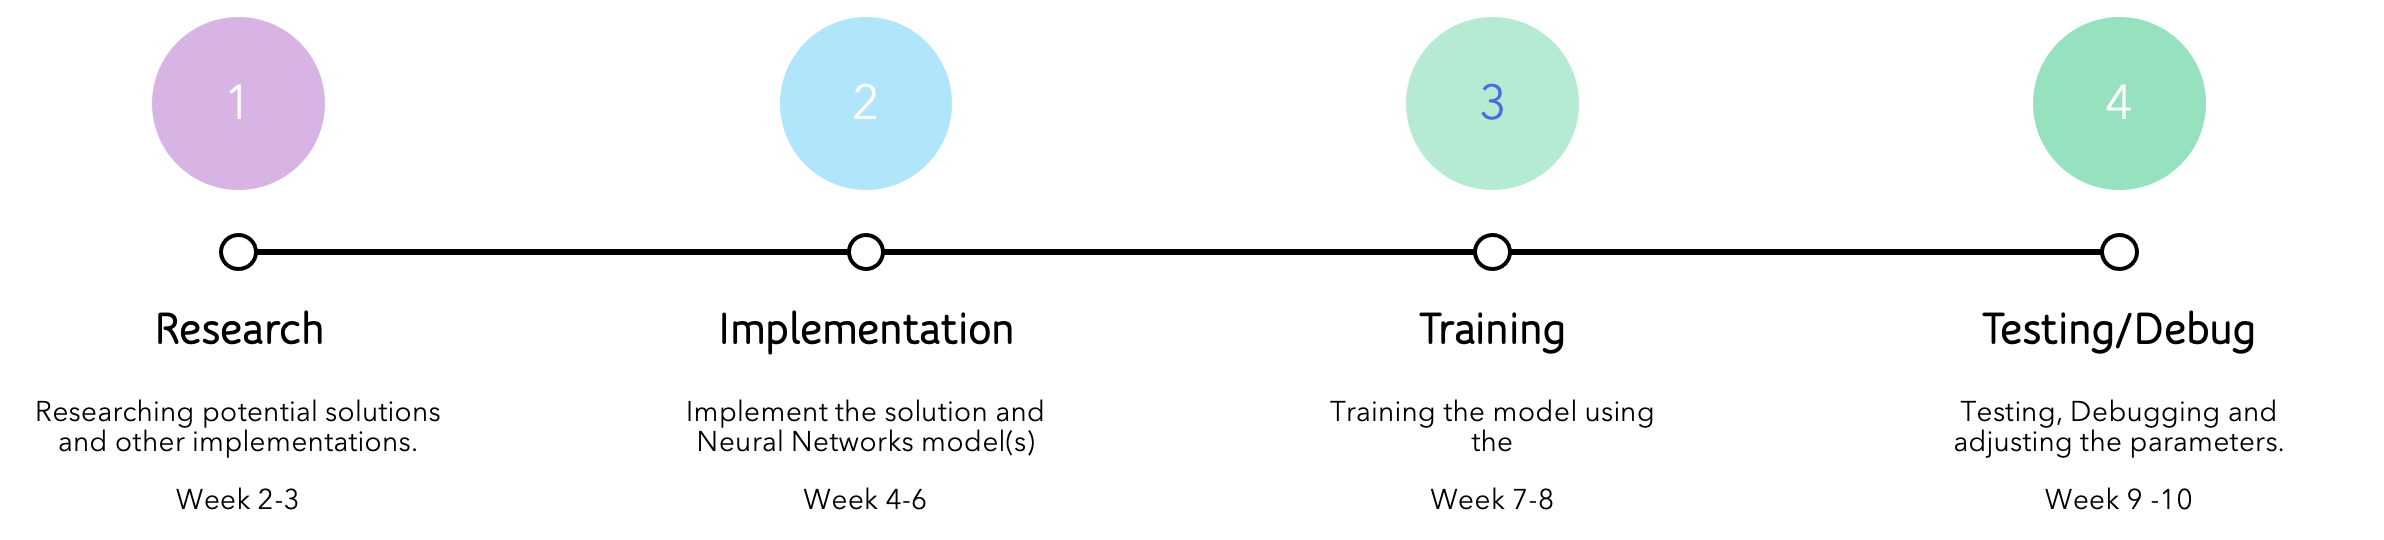
\includegraphics[width=\textwidth]{timeline.png}
\end{figure}

\section{Method}
\subsection{The Pipeline}
The present study aims to use a dataset comprising of underexposed images, which are paired with corresponding longer exposure images that serve as the ground truth. Specifically, the See-In-The-Dark (SID) dataset, consisting of approximately 5,000 high resolution images, will be utilized. The SID dataset comprises of 5094 raw short-exposure images, each paired with a reference long-exposure image. It is important to note that each long-exposure image is paired with multiple short-exposure images. 

To achieve our objective of direct single image processing of fast low-light images, we propose to utilize end-to-end learning. This will be accomplished through training a variational autoencoder (VAE) in conjunction with a convolutional neural network (ConvNet) proposed in paper SIG \cite{LearningToSeeInTheDark} to perform the entire image processing pipeline. The VAE will be responsible for providing artistic enhancements to the images, while the ConvNet will be utilized to recover the high frequency details from the low signal-to-noise ratio (SNR) image. The ConvNet will be implemented using U-Net architecture. % More explaination on U-Net

The output from the VAE and the ConvNet will be summed together and then passed through a discriminator network. 

\subsection{Training}
KL divergence can be used as a loss function to train the variational autoencoder (VAE) in our proposed method of end-to-end learning for direct single image processing of fast low-light images. In this section, we will discuss how we will incorporate KL divergence into the training process.

The KL divergence is a measure of the difference between two probability distributions. In our case, we will use it as a measure of the difference between the distribution of the encoded latent variables produced by the VAE and the standard normal distribution. The goal of incorporating KL divergence into the loss function is to encourage the VAE to learn a compact and smooth representation of the input data.

During training, we will minimize the sum of two losses: the reconstruction loss and the KL divergence loss. The reconstruction loss measures the difference between the input image and the output image generated by the VAE, and it is commonly implemented using pixel-wise mean squared error. The KL divergence loss measures the divergence between the distribution of the latent variables and the standard normal distribution.

The total loss function can be expressed as:

\begin{equation}
    L_{total} = L_{recon} + \beta * KL_{div}
\end{equation}

where $L_{recon}$ is the reconstruction loss, $KL_{div}$ is the KL divergence loss, and $\beta$ is a hyperparameter that controls the importance of the KL divergence loss relative to the reconstruction loss.

During training, we will update the weights of the VAE using backpropagation to minimize the total loss function. By minimizing the KL divergence loss, we will encourage the VAE to learn a more compact and smooth representation of the input data, which will in turn lead to better image quality.

In summary, we will incorporate KL divergence as a loss function in our training process to encourage the VAE to learn a more compact and smooth representation of the input data. This will improve the overall image quality of the output generated by the VAE.

\section{Algorithm}
\subsection{Inputs}

    \begin{itemize}
        \item Pair of Low Signal-to-Noise image and its corresponding high Signal-to-Noise image as ground truth
        \item Hyperparameters (learning rate, number of epochs, batch size, etc.)
    \end{itemize}

\subsection{Outputs}
    \begin{itemize}
        \item Processed images with artistic enhancements and boosted Signal-to-Noise ratio
    \end{itemize}

\subsection{Procedure}
    \begin{enumerate}
    
    \item Load the dataset of underexposed images with corresponding ground truth long-exposure images.
    
    \item Split the dataset into training and testing sets.
    
    \item Initialize the variational autoencoder network, ConvNet in U-net structure from SID and train both networks in parallel with the following steps:
    \begin{enumerate}
        \item Variational autoencoder network (VAE-Net):
        \begin{enumerate}
            \item Forward pass the underexposed images $I_U$ through the variational autoencoder (VAE) consist of convolution layers to learn the noise distribution from input images, $\mu$ and $\sigma$
            \item Decoder from VAE samples from the learned distribution and output pixel level enhancement map, $D$.
        \end{enumerate}
        \item ConvNet:
        \begin{enumerate}
            \item Forward pass the underexposed image $I_U$ through the ConvNet to obtain boosted Signal-to-Noise ratio image, $B$.
            \item Calculate the L2 loss between the recovered the boosted Signal-to-Noise ratio image from step (i) and its corresponding ground truth long-exposure images, $I_T$.
            \item Backward propagate the L2 loss into ConvNet.
        \end{enumerate}
    \end{enumerate}
    
    \item After obtaining the pixel level enhancement map $D$ and boosted Signal-to-Noise ratio image $B$, we sum up both of them pixel by pixel to obtain the output image $O = \sum_{(x,y)\in I_U}D_{x,y} + B_{x,y}$.

    \item Forward pass the output image $O$ and corresponding ground truth $I_T$ into discriminator, obtain a single scalar representing whether our network output is real or fake, and calculate adversarial loss $L_{adv}$.

    \item Back-propagate adversarial loss $L_{adv}$ into discriminator network

    \item Calculate Joint loss $L_{Joint}$ of L2 loss $L_{D}$ between VAE-Net output $O$ and corresponding ground truth $I_T$, adversarial loss $L_{adv}$, and KL divergence $KL(N(\mu, \sigma), N(0, 1))$. $L_{Joint} = L_{D} + L_{adv} + KL(N(\mu, \sigma), N(0, 1))$, 
    
    where $KL(N(\mu, \sigma), N(0, 1)) = \log \frac{1}{\sigma} + \frac{\sigma^2 + \mu^2}{2} - \frac{1}{2}$ \cite{PytorchVAE}

    \item Back-propagate Joint loss $L_{Joint}$ into VAE-Net.

    \end{enumerate}

    %Objective Function
    
    At the end of training, freeze the weights of the variational autoencoder and the U-net for future inference purpose.
    During inference, we use the trained model to forward passing underexposed images into both variational autoencoder and U-net, and the sum of both outputs will be the final output from our proposed network with artistic enhancements and recovered well-exposed image.
    
\begin{figure}[h]
  \centering
  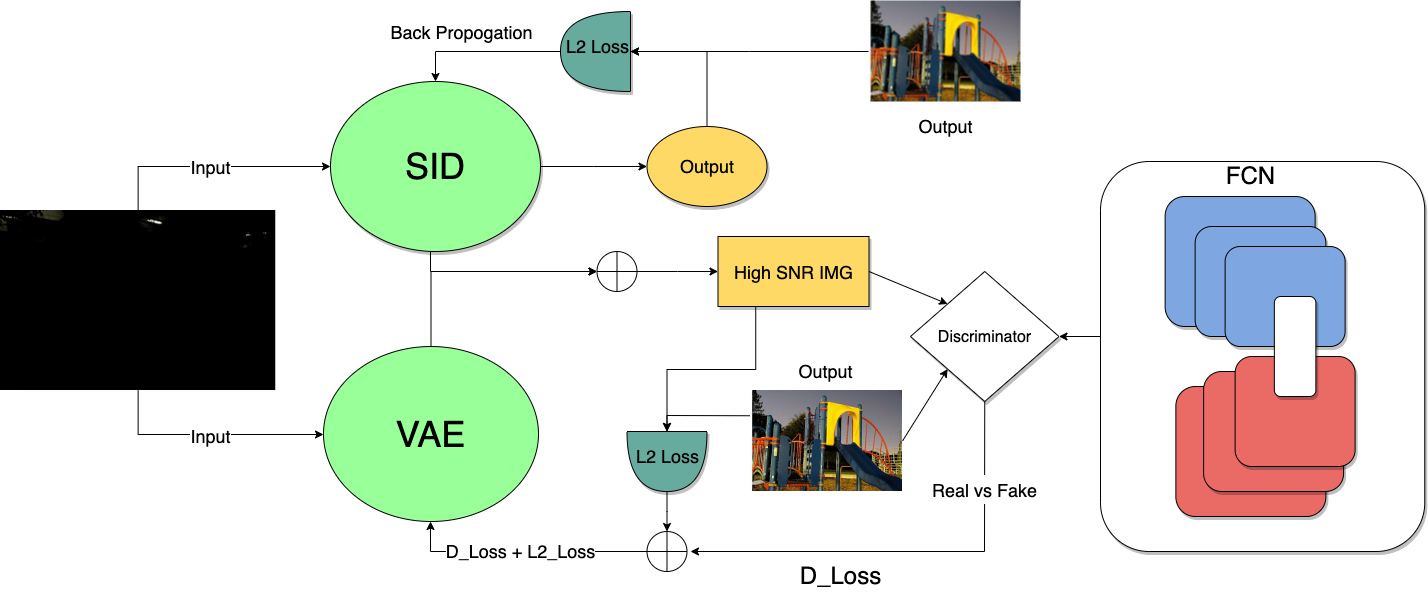
\includegraphics[width=\textwidth]{VAE Diagram.drawio.png}
\end{figure}



\section{Theory}
The proposed method for direct single image processing of fast low-light images involves the use of advanced deep learning techniques, specifically, a U-Net architecture. The U-Net is a convolutional neural network that has been shown to be effective in image segmentation \cite{UNetBasedMedicalImageSegmentation} and other image processing tasks. 

In this approach, the U-net is used to improve the image quality of underexposed images while recovering the ground truth data. The U-net is trained on a dataset of paired under-exposed and well-exposed images, where the low-light image is the input, and the high-light image is the ground truth. The U-Net learns to map the low-light image to the high-light image, recovering the lost information due to the low signal-to-noise ratio.

To further enhance the overall image quality, the U-Net is trained in conjunction with a generative model, such as a variational autoencoder (VAE). The VAE is used to provide artistic enhancements to the underexposed images, such as adjusting the brightness, contrast, and color saturation. The VAE is trained on a large dataset of high-quality images and then used to enhance the underexposed images.

To optimize the overall image quality, the U-Net and VAE are trained in parallel, allowing the VAE to improve the overall appearance of the image, while the U-Net improves the accuracy of the image. The loss function used to train the model combines the objectives of the U-Net and VAE, encouraging the model to produce high-quality images that are close to the ground truth.

The model is trained on a dataset of paired short-exposure and long-exposure images, allowing the model to learn from multiple examples of the same ground truth data. Finally, the output of the U-Net and VAE are combined and evaluated using a discriminator network to ensure that the final image is of high quality.




\medskip
\printbibliography %Prints bibliography
\end{document}